\documentclass{article}
\usepackage[utf8]{inputenc}
\usepackage[english]{babel}

\textwidth 16.2cm \textheight 23cm \topmargin -0.6cm
\oddsidemargin 0.31cm \evensidemargin -0.91cm

\usepackage{natbib}
\usepackage{amsmath}
\usepackage{amsfonts}
\usepackage{amsbsy}
\usepackage{amssymb}
\usepackage{algorithm2e}
\usepackage{graphicx}
\usepackage{psfrag}
\usepackage{epsfig}
\usepackage{multicol}
\usepackage{cite}
\usepackage{color}
\usepackage{dsfont}
\usepackage[center]{caption}
\usepackage{listings} 
\usepackage{xcolor} 
\usepackage{textcomp}
\usepackage{hyperref}

\hypersetup{
    bookmarks=true,         % show bookmarks bar?
    unicode=false,          % non-Latin characters in Acrobat’s bookmarks
    pdftoolbar=true,        % show Acrobat’s toolbar?
    pdfmenubar=true,        % show Acrobat’s menu?
    pdffitwindow=false,     % window fit to page when opened
    pdfstartview={FitH},    % fits the width of the page to the window
    pdftitle={My title},    % title
    pdfauthor={Author},     % author
    pdfsubject={Subject},   % subject of the document
    pdfcreator={Creator},   % creator of the document
    pdfproducer={Producer}, % producer of the document
    pdfkeywords={keyword1} {key2} {key3}, % list of keywords
    pdfnewwindow=true,      % links in new window
    colorlinks=true,       % false: boxed links; true: colored links
    linkcolor=blue,          % color of internal links (change box color with linkbordercolor)
    citecolor=blue,        % color of links to bibliography
    filecolor=magenta,      % color of file links
    urlcolor=cyan,           % color of external links
	pdfborder	= {0 0 0}
}

\def\endproof{\hfill $\Box$\newline\newline}
\def\proof{\par\noindent{\it Proof}. \ignorespaces}

\newcommand{\RR}{\mathbb{R}}
\newcommand{\qr}{\textrm{QsRank}}

\title{Qs Rank and efficient $\epsilon$-neighbor search}
\author{Arthur Darcet \& Yohann Salaun}
\date{\today}

\parindent=0pt
\begin{document}
\maketitle

\section{Overview}

The QsRank algorithm, described in \citep{QSRank}, is a method that allows a ranking for binary hash codes to efficiently perform $\epsilon$-neighbors search in large data. The aim of this problem is to, for a given query $q$ and a given radius $\epsilon$, quickly finds the data subset $Y = (y_i)_i$ such that $\forall i,\  ||y_i-q|| < \epsilon$.\\
Methods based on the Hamming distance have been recently developed to solve efficiently such a problem for large data. However these latter methods often lack of precision due to their binarization of the query which induces a lack of speed in the performances of their algorithm. The methods presented here, performs a more accurate ranking for hash codes and thus allows a faster and more efficient method for $\epsilon$-neighbors retrieval.

\section{Theoretical Description}

The algorithm of $\epsilon$-neighbor search using the QsRank works in two times:
\begin{itemize}
	\item[\textbf{1.}] Hash code generation of the data for faster retrieval
	\item[\textbf{2.}] Ranking of the hash code depending on a query
\end{itemize}
The first part can be computed before any requests whereas the second needs the parameters of the search (query $q$ and neighbor distance $\epsilon$).

\subsection{Hash Codes generation}

Such search algorithm are used for huge data with components in high dimensional space. Thus, in order to generate simple hash codes for each input data point $x \in \RR^d$, a Principal Component Analysis (PCA) is computed.\\
The hash code $h$ of $x$ is then computed by taking the sign of the PCA-projections:
\[	
\forall j \in [1;d],\ h_j = 	
 	\left \{
		\begin{array}{c}
    		1 \text{ if }(PCA(x, \{x_i\}_i))_j > 0 \\
    		0 \text{ if }(PCA(x, \{x_i\}_i))_j \leq 0
		\end{array}
	\right.
\]
In practice, only the first components of the hash codes are computed.\\
The benefits given by the PCA are numerous:
\begin{itemize}
	\item[\textbf{1.}] The PCA allows a dimension decrease but keeps most of the information. This way, hash codes are shorter and the retrieval is still efficient.
	\item[\textbf{2.}] The PCA is an orthogonal projection that preserves the $L^2$-norm. Thus, the $\epsilon$-ball around a query is still meaningful after PCA.
	\item[\textbf{3.}] The PCA values of the input data points are uncorrelated which will lead to an efficient ranking with Qs Rank.
\end{itemize}

\subsection{QsRank for Hash Codes ranking}

We suppose, that the projection $y$ of the input data points $x$ are distributed along a probability distribution function $p$. Then, with a given query $q$, a neighbor distance $\epsilon$ and a hash code $h$, the Qs Rank formula is defined by:
\[
	\qr(q, h, \epsilon) = \frac{\int_{NN(q,\epsilon) \cap S(h)} p(y) dy}{\int_{NN(q,\epsilon)} p(y) dy}
\]
where:
\begin{enumerate}
	\item[$\bullet$]$NN(q,\epsilon) = \{y \in \RR^d \text{ s.t. } ||y-q||<\epsilon\}$ is the $\epsilon$-ball around the query $q$
	\item[$\bullet$]$S(h) = \{y \in \RR^d \text{ s.t. } \forall i \in [1;d] y_i h_i > 0 \}$ is the set described by the hash code $h$
\end{enumerate}

The QsRank can only be seen as a probability, with Bayes rule:
\[
	\qr(q, h, \epsilon) = \frac{\mathbb{P}(y\in NN(q,\epsilon) \cap S(h))}{\mathbb{P}(y\in NN(q,\epsilon))} = \mathbb{P}(y \in S(h) | y\in NN(q,\epsilon))
\]
Thus, the QsRank only ranks hash codes with respect to their probability of containing many $\epsilon$-neighbors.

\subsection{QSRank approximation}

In order to compute fast retrieval, the QsRank will be approximated by a lighter formula.\\
First, only the top $k$ dimensions of the PCA projection will be used ($k$ will be defined afterward in the next section). Thus, $NN(q,\epsilon)$ becomes $NN(q^k,\epsilon)$ and $S(h)$ becomes $S(h^k)$ where $x^k$ is the k-top dimensions of a vector $x \in \RR^d$. This approximation seems legit since the aim of the PCA is to find the dimensions where most of the information is kept.
\[
	\qr(q, h, \epsilon) \approx \frac{\int_{NN(q^k,\epsilon) \cap S(h^k)} p(y^k) dy^k}{\int_{NN(q^k,\epsilon)} p(y^k) dy^k}
\]
Another approximation is to replace the $\epsilon$-ball by an $\epsilon$-hypercube:
\[
	NN(q^k,\epsilon) \leftrightarrow HC(q^k,\epsilon) = \{y^k \in \RR^k \text{ s.t. } \forall i \in [1;k], |y^k_i-q^k_i|<\epsilon\}
\]
Moreover, since the PCA produces uncorrelated projections, each dimension of $p(y)$ is supposed to be independent. The QsRank approximation then becomes:
\[
	\qr(q, h, \epsilon) \approx \prod_{i=1}^k \frac{\int_{|y^k_i - q^k_i| < \epsilon, y^k_i h^k_i > 0 } p(y^k_i) dy^k_i}{\int_{|y^k_i - q^k_i| < \epsilon} p(y^k_i) dy^k_i} = \prod_{i=1}^k \mathbb{P}(y^k_i \in S(h^k_i) | y^k_i \in HC(q^k_i,\epsilon))
\]
The last approximation is to consider that the $y$ are generated from a uniform law. This assumption accelerates a lot the computation and seems to work quite well in accordance with the authors of \citep{QSRank}. The final formula thus becomes:
\begin{eqnarray*}
	\qr(q, h, \epsilon) 
	& \approx & \prod_{i=1}^k \frac{\int_{|y^k_i - q^k_i| < \epsilon, y^k_i h^k_i > 0 } dy^k_i}{\int_{|y^k_i - q^k_i| < \epsilon} dy^k_i} \\
	& \approx & \prod_{i=1}^k \text{clamp} \left(\frac{1}{2}\left( 1 + \frac{h^k_i q^k_i}{\epsilon} \right), [0;1] \right)                  
\end{eqnarray*}

Opposed to the Hamming distance, this measure has many substantial advantages :
\begin{enumerate}
	\item[$\bullet$] The radius $\epsilon$ is took into account	
	\item[$\bullet$] Since it is a product, if one of the component of the hash code induces a null probability, the whole QsRank becomes null. Some sets are thus not explored whereas Hamming distance methods would have.
\end{enumerate}

\section{Implementation}

\subsection{Efficient computation}

Once the query $q$ is given, the logarithmic QsRank is computed for the $2^k$ different hash codes. This results in $\mathcal{O}(k)$ logarithm computation and $\mathcal{O}(k 2^k)$ additions. Moreover, only hash codes with non zeros probabilities have to be computed, which accounts for only $15\%$ of the data points according to the experiments made in \citep{QSRank}.\\
The idea of the retrieval is also to make a pre-selection with QsRank computed only on the first $K_1$ bits. Then, the $L$ first buckets are selected and more accurate re-ranking (on $K_1+K_2$ bits) is computed to select the $\epsilon$-neighbors.

\begin{figure}[htbp]
	\begin{center}
	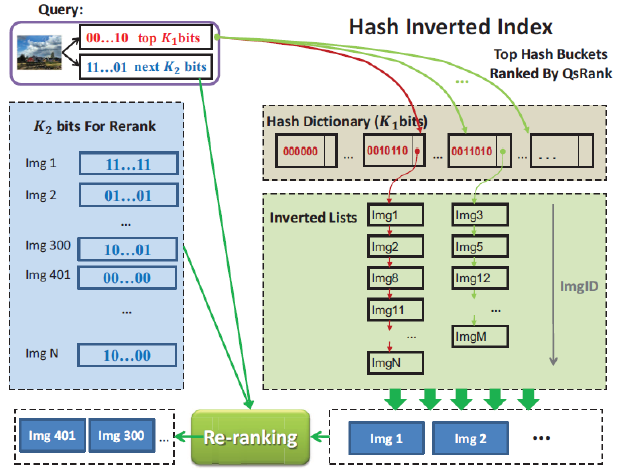
\includegraphics[width=.6\linewidth]{Images/algo.png}
	\caption{Retrieval procedure: Buckets ranking ($K_1$ bits). Neighbors re-ranking ($K_1+K_2$ bits). Image credits from \citep{QSRank}}
	\end{center}
	\label{fig:algo}
\end{figure}

\subsection{Retrieval procedure}

\begin{algorithm}[H]

\textbf{Input} : input data $X \in \RR^{n \times d}$, query $q$, radius $\epsilon$\\
\textbf{Parameters}: hash codes length $K_1$ and $K_2$, number of buckets $L$.\\
\textit{Precomputation}\\
$Y = PCA(X)$\\
\For{$i=1~..~K_1+K_2$}{
	\textbf{Compute} the logarithmic sub-QsRanks : $\log\left(\text{clamp} \left(\frac{1}{2}\left( 1 + \frac{h^k_i q^k_i}{\epsilon} \right), [0;1] \right)\right)$
}
\textit{$\epsilon$-search}\\
\textbf{Sort} the buckets by $K_1$-QsRank.\\
\textbf{Pick} the $L^{th}$ first buckets.\\
\textbf{Sort} the buckets hash codes by $(K_1+K_2)$-QsRank.\\
\textbf{Return} the $\epsilon$-neighbors.
\end{algorithm}

\subsection{Implementation details}
Our implementation use \textit{Matlab} with the statistic toolbox.
The script \verb=main.m= contains an exemple search in data points loaded from \verb=data/feat_oxc1_hesaff_sift.bin=\footnote{Download from \url{http://www.robots.ox.ac.uk/~vgg/data/oxbuildings/feat_oxc1_hesaff_sift.bin.tgz} and unzip to data/}.\\

The script \verb=recall_graph.m= was used to generate the two recall-loss graph that are presented in this report.\\

And the script \verb=demo2d.m= show the first two steps of the algorithm (PCA and $K_1$-QsRank separation) in $2D$\\


\section{Results}

We have implemented the algorithm the way it is explained above. The parameters used are the one proposed in \citep{QSRank}. They are summed up in the table below.
\begin{table}[htbp]
\begin{center}
  \begin{tabular}{|c|c|c|}
		\hline
		$K_1$ & $K_2$ & L \\
		\hline
		16 & 48 & 50\\
		\hline
\end{tabular}
\caption{Default parameters used for the algorithm.}
\end{center}
\label{tab:params}
\end{table}

Then, in order to evaluate its efficiency, we have generated many queries and compared the results obtained by the algorithm and the true neighbors with the \textit{recall loss}:
\[
	r_{loss} = \frac{|\text{found neighbours}|}{|\text{true neighbours}|}
\]
The results can be observed on figure \ref{fig:rloss}

\begin{figure}[htbp]
	\begin{center}
	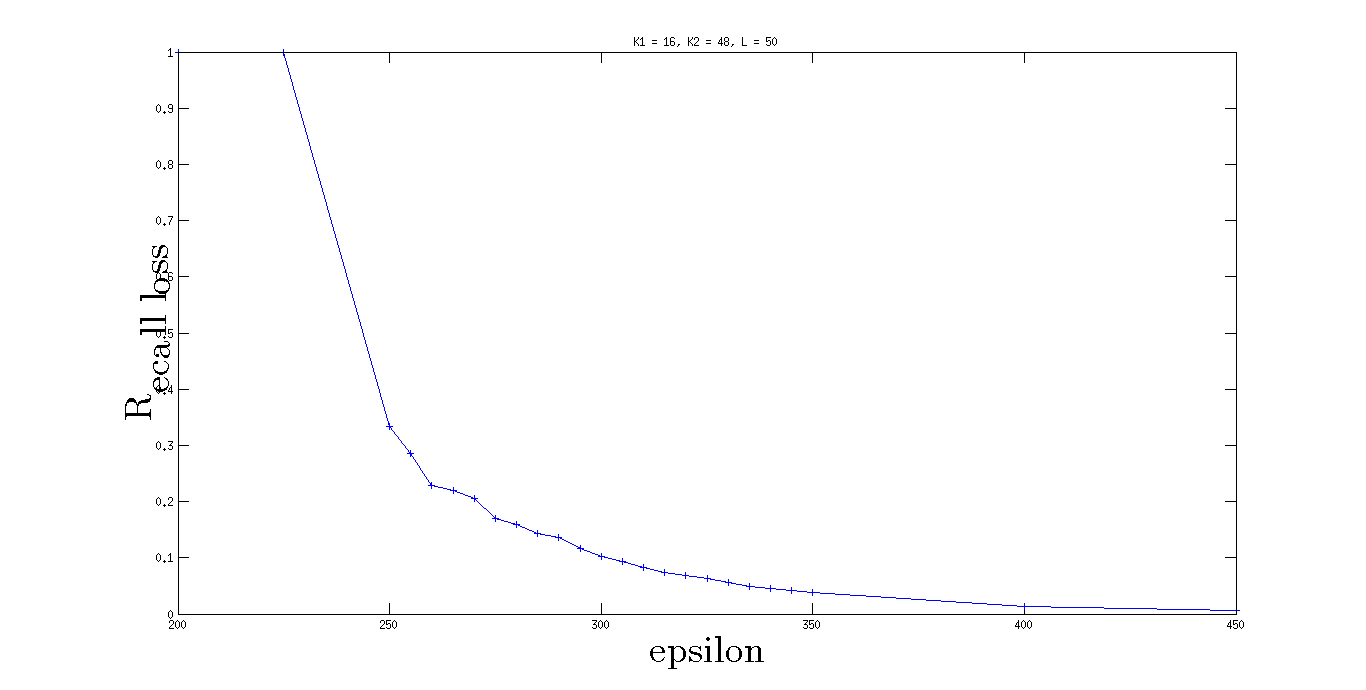
\includegraphics[width=.8\linewidth]{Images/rloss.png}
	\end{center}
	\caption{Recall Loss function of epsilon.}
	\label{fig:rloss}
\end{figure}

This graph shows that $\epsilon$ needs not to be too high in order to keep the approximations made in the previous sections correct. Otherwise, the results are quickly inaccurate.

\begin{figure}[htbp]
	\begin{center}
	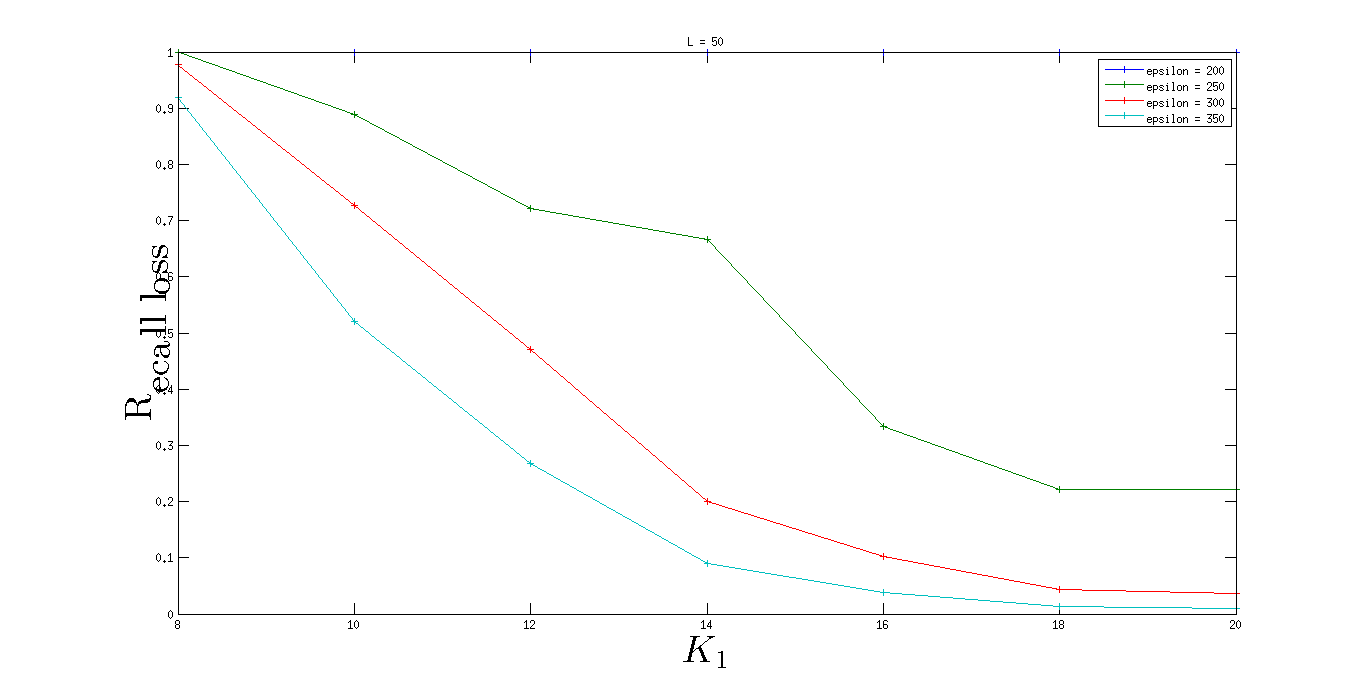
\includegraphics[width=.8\linewidth]{Images/k1_rloss.png}
	\end{center}
	\caption{Recall Loss function of $K_1$.}
	\label{fig:k1_rloss}
\end{figure}

We can also observe, in figure \ref{fig:k1_rloss}, the loss as a function of $K_1$: when $K_1$ get higher, the number of buckets increase and the average number of points per bucket decrease. With a fixed number $L$ of buckets selected, the number of points that are considered irrelevant by the algorithm after the $K_1$-QsRanking increase when $K_1$ decrease. This explain why the loss is inversely proportional to $K_1$.\\

Although, the algorithm seems to have good speed performances ($\sim 0.2s$ according to \citep{QSRank}), ours is not as fast. This could be explained by the use of the \textit{Matlab} software and the hashmap generations that seems to take too much time (\textit{Matlab} require our algorithm to convert back and forth between table of $-1$ and $1$ and \textit{uint64} to represent the hashcodes. This shouldn't be necessary).\\


\section{Conclusion}

With this article, we have discovered the field of large-scale-$\epsilon$-neighbors search. A field that becomes more and more significant because of the huge increase of available data on the internet. The method presented in \citep{QSRank} differs a lot from the other state-of-the-art ones by not using the Hamming distance for the retrieval. It induces a better precision for the search. Moreover, the number of bits used is much smaller (only 64 bits) which reduces memory cost speed up the process. However, this number is not very movable since it depends on the PCA and thus on the initial dimension of the space.\\
Finally, this method is powerful by its simplicity and efficiency. Many approximations are made to make this algorithm fast but it is still very efficient as it is equal to other state-of-the-art methods.

\bibliographystyle{plain} %Style of Bibliography: plain / apalike / amsalpha / ...
\bibliography{literature} %You need a file 'literature.bib' for this.

\end{document}
